\section{Information-Capacity Framework}
\label{sec:info-bound}

We derive an information-theoretic upper bound on the test accuracy of an
$N$-qubit variational quantum circuit (VQC) router on a $K$-class task,
combining the Holevo bound on classical-information extraction from quantum
measurements~\cite{holevo1973bounds} with Fano's inequality~\cite{fano1961transmission}.

\subsection{Setup}

The routing architecture is (i) a frozen pretrained encoder $\phi : \mathcal{T} \to \mathbb{R}^{d}$
(here MiniLM-L6-v2, $d=384$), (ii) a learned projection $\pi_\theta : \mathbb{R}^d \to \mathbb{R}^{N}$
with $\pi_\theta(x) = \pi \cdot \tanh(W x + b)$, (iii) an $N$-qubit variational
circuit producing measurements $M = (\langle Z_1 \rangle, \ldots, \langle Z_N \rangle)
\in [-1, 1]^N$, and (iv) a linear classifier $\sigma_\psi : \mathbb{R}^N \to \Delta^{K-1}$
producing class probabilities. The end-to-end function $f : \mathcal{T} \to \{1, \ldots, K\}$
is $\mathop{\arg\max} \circ \sigma_\psi \circ M \circ \pi_\theta \circ \phi$.

\subsection{Holevo capacity}

For any POVM $\{E_M\}$ measurement on an $N$-qubit state and any classical variable
$Y$, the Holevo bound~\cite{holevo1973bounds} states
\begin{equation}
I(M; Y) \leq S(\rho_Y) \leq N,
\label{eq:holevo}
\end{equation}
where $S$ is the von Neumann entropy. For our measurement (single-qubit $Z$
expectations on a joint state), $I(M; Y)$ is at most $N$ bits regardless of
the input distribution. At $N = 4$: at most 4 bits of class information
flow from the circuit to the classifier.

\subsection{Fano's inequality}

Given any classifier $\hat{Y}$ of $Y$ over $K$ classes from an observation
$M$, Fano's inequality~\cite{fano1961transmission} gives
\begin{equation}
P_\mathrm{err} \geq \frac{H(Y) - I(M; Y) - 1}{\log_2(K - 1)}.
\label{eq:fano}
\end{equation}
With uniform prior, $H(Y) = \log_2 K$. At $K = 10$: $H(Y) \approx 3.32$ bits.

\subsection{Combined bound}

Substituting~\eqref{eq:holevo} into~\eqref{eq:fano}:
\begin{equation}
\mathrm{acc}_\mathrm{max}(N, K, I) = 1 - \frac{\max(0, \log_2 K - \min(I, N) - 1)}{\log_2(K - 1)}.
\label{eq:bound}
\end{equation}
This is monotone non-decreasing in $I$ up to the Holevo cap $N$: additional
embedding information beyond $N$ bits cannot improve the VQC's accuracy, as
it cannot fit through the $N$-qubit measurement channel.

\subsection{Numerical verification}

We estimate $I(X_{\mathrm{PCA}(d)}; Y)$ on our 10-class routing task using the
Kraskov-Stögbauer-Grassberger $k$-NN estimator~\cite{kraskov2004estimating}
implemented in scikit-learn's \texttt{mutual\_info\_classif}, for
$d \in \{2, 4, 8, 16, 32, 64, 128, 384\}$. Figure~\ref{fig:bound} (panel A)
shows the estimated $I$ at each dimension alongside the Holevo cap for $N=4$
qubits and $H(Y) = \log_2 10$. Panel B plots the Fano-derived upper bound at
each dim alongside our empirical C1 accuracies.

At $d = 4$ (information-matched to our VQC), the estimated MI is
$2.04$ bits. Equation~\eqref{eq:bound} then gives
$\mathrm{acc}_\mathrm{max} \approx 0.911$ as an upper bound on
the test accuracy of any 4-qubit VQC on this task. Our measured VQC accuracy
of $0.246 \pm 0.031$ falls well under this bound, consistent with (but far
from saturating) the theoretical ceiling.

\begin{figure}[tb]
  \centering
  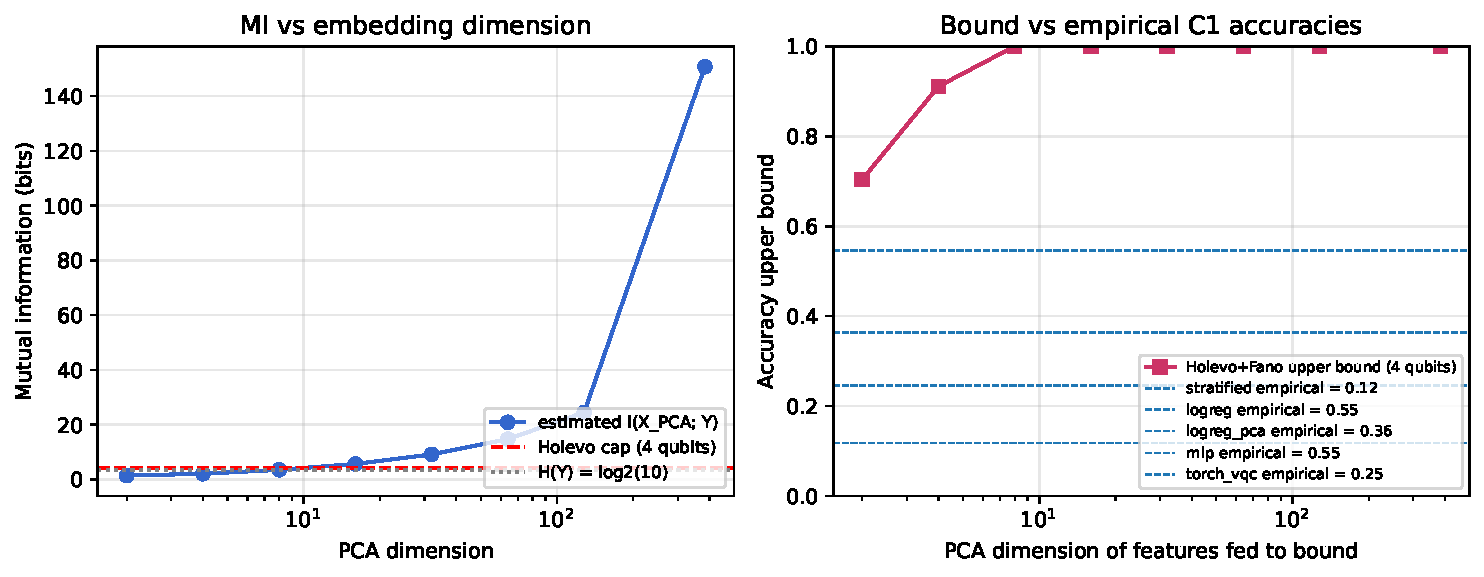
\includegraphics[width=\linewidth]{c5-bound-figure.pdf}
  \caption{Left: estimated mutual information between PCA-compressed embeddings
    and class labels, for embedding dimensions 2 to 384. Red dashed line marks
    the Holevo cap for 4 qubits; grey dotted line marks $H(Y) = \log_2 10$.
    Right: Fano+Holevo upper bound on accuracy for a 4-qubit VQC as a function
    of the projected-dimension's MI, with empirical C1 classifier accuracies as
    horizontal references.}
  \label{fig:bound}
\end{figure}

\subsection{What the bound does NOT say}

The bound~\eqref{eq:bound} is necessary, not sufficient. Reaching
$\mathrm{acc}_\mathrm{max}$ requires (i) a projection $\pi_\theta$ that
preserves all the class-relevant information in $X$, and (ii) a circuit +
measurement that achieves the Holevo cap. Neither is automatic: the naive
$\pi \tanh$ projection saturates and destroys signal, and the expressivity of
\texttt{StronglyEntanglingLayers} with $\langle Z \rangle$ measurement is
bounded by MPS bond-dimension-equivalent results (Du et al.~\cite{du2020expressive},
Theorem 4: deep circuits with bond dimension $D$ are covered by
$\mathcal{O}(\mathrm{poly}(\log D))$ Pauli-$Z$ expectation-value blocks). The
large gap between our measured $0.246$ and the theoretical ceiling $0.911$
therefore reflects projection and measurement sub-optimality rather than a
fundamental quantum-information limit. Closing this gap is the subject of
ongoing architectural work.
